\documentclass[conference]{IEEEtran}
\IEEEoverridecommandlockouts
\usepackage[utf8]{inputenc}
\usepackage{cite}
\usepackage{amsmath,amssymb,amsfonts}
\usepackage{graphicx}
\usepackage{textcomp}
\usepackage{xcolor}
\usepackage{subcaption}
\usepackage{stfloats}   
\usepackage{placeins}   
\usepackage{multirow}

\def\BibTeX{{\rm B\kern-.05em{\sc i\kern-.025em b}\kern-.08em
    T\kern-.1667em\lower.7ex\hbox{E}\kern-.125emX}}

\begin{document}
\renewcommand{\topfraction}{0.9}
\renewcommand{\bottomfraction}{0.9}
\renewcommand{\textfraction}{0.07}
\renewcommand{\floatpagefraction}{0.7}
\renewcommand{\dblfloatpagefraction}{0.7}
\renewcommand{\dbltopfraction}{0.9}
\setcounter{topnumber}{4}
\setcounter{bottomnumber}{4}
\setcounter{totalnumber}{8}
\setcounter{dbltopnumber}{4}

\title{Beyond Screen Time: A Machine Learning Framework for Predicting Student Academic Risk from Gaming Habits}

\author{
\IEEEauthorblockN{Afnan Mohammad Hafiz}
\IEEEauthorblockA{
\textit{Department of Computer Science and Engineering} \\
\textit{BRAC University} \\
Dhaka, Bangladesh \\
afnan.mohammad.hafiz@g.bracu.ac.bd}
\and
\IEEEauthorblockN{Ibsan Hossain Ansari}
\IEEEauthorblockA{
\textit{Department of Computer Science and Engineering} \\
\textit{BRAC University} \\
Dhaka, Bangladesh \\
ibsan.hossain.ansari@g.bracu.ac.bd}
}

\maketitle

\begin{abstract}
With the rise of online gaming, students have become a growing concern about its impact on their academic work, especially if they are playing too much or too often. In this study, the relationship between gaming habits, lifestyle factors, and academic performance is explored through machine learning approaches. The dataset included 250 anonymous gamer profiles with 49 attributes, including characteristics, gaming habits, psychological factors, well-being measures, and academic results. Exploratory analysis revealed that there was a very skewed distribution of academic performance scores, with the majority of observations falling into the highest academic performance score category. Features that did not contribute to the prediction of the problem were eliminated, missing data were filled in using imputation, and the GPA scores were binned into three performance categories: low, medium, or high. The minority classes were then oversampled to obtain a balanced training set. The features were standardized, and 19 components were retained after Principal Component Analysis to capture most of the variance. The classification models used were trained using an 80/20 train-test split as follows: Decision Tree, Logistic Regression, Random Forest, XGBoost, Support Vector Machine (SVM), a Neural Network (Multi-Layer Perceptron) and Gradient Boosting. The accuracy, precision, recall, F1 score, AUC-ROC, and confusion matrix were used to assess the model performances. XGBoost outperformed all other seven classifiers with an overall accuracy of 76\%, followed closely by Gradient Boosting and Random Forest with 75\% and 74\% accuracy, respectively. The study also reveals the potential of machine learning in examining the aspects of gaming and how it can classify students based on their academic performance levels, highlighting the difficulties of unbalanced academic data and the complex connection between gaming conduct and academic results.
\end{abstract}

\begin{IEEEkeywords}
predictive modeling, machine learning, student risk, gaming habits, data analysis, academic performance
\end{IEEEkeywords}

\section{Introduction}
Smartphones, high-speed Internet, and convenient online gaming have made video games a way of life for students. Although gaming can be an entertaining and therapeutic experience in reasonable amounts, the excessive or addictive use of gaming can be associated with various negative aspects, including sleep deprivation, less study time, attendance problems at school, decreased motivation, and poor academic performance (GPA, CGPA, etc.). However, the current studies on the relationship between gaming addiction and academic outcomes tend to be descriptive or have small and limited numbers of participants in a single institution, and the results have been inconsistent; some report negative effects, while others report insignificant or even positive effects.

There is a gap in the literature for a predictive, data-driven approach for modelling the relationship between gaming behaviour, demographic and lifestyle factors, and academic performance on a large scale. This project fills this void by leveraging machine learning (supervised learning) techniques on a structured dataset of student gaming habits and academic outcomes, looking for the key behavioral patterns that predict poor academic performance, and creating models that can detect at-risk students early.

\section{Literature Review}

\subsection{Gaming Addiction, Internet Use, and School Engagement}
Studies examining gaming and academic performance typically place the issue of gaming in the context of Internet addiction. Ta\c{s} \cite{tas2019} conducted a study with 365 high school students in Turkey who filled out validated addiction and engagement scales and analyzed them with Pearson correlation and multiple regression. It revealed that there was a slight, but significant negative correlation between Internet addiction and school engagement, and that there was no significant correlation between gaming addiction and school engagement; the two combined accounted for approximately 4\% of the variance. The study has limited generalizability due to its single-school, cross-sectional, self-report design, and the lack of previous studies that examine the link between gaming addiction and school engagement is notable.


\subsection{Gaming and Academic Performance in Western Contexts}
Wright \cite{wright2011} analyzed 198 U.S. college students, conducting one-way ANOVAs to determine if differences existed between the GPA of players and non-players and testing for correlations with weekly playtime. The study revealed a significant difference between player and non-player group GPAs, with an average lower GPA for players compared to non-players, but no significant correlation between hours played or puzzle/strategy exposure with GPA. Self-reported GPA and a single-institution sample (homogeneous), along with an unvalidated researcher-designed survey, were limitations. Overall, Wright's results support a general trend in the literature with positive, negative, and neutral associations between gaming and academic outcomes, and highlight the need for more longitudinal studies and measures of engagement.

\subsection{Gaming and Academic Performance in South Asian Contexts}
A few studies have specifically examined the population of South Asian students. They surveyed 399 students from three Bangladeshi universities and performed chi-square tests and logistic regression between video game time, absence from class, and the demographics of the students and their CGPA, as reported by Mahmud et al. (2020) \cite{mahmud2020}. The researchers concluded that those who played 30 or more hours a week had a significantly greater risk of poor academic performance (CGPA), and that skipping classes and the number of hours spent studying were also significant factors. In the same way, Anjum et al. \cite{anjum2021} conducted a cross-sectional survey of school-going adolescents in Bangladesh and reported a strong negative correlation between severe gaming addiction and learning outcomes, which is explained by sleep disturbance, fatigue, and loss of motivation due to late hours of gaming. Both studies used cross-sectional, self-reported data and had limitations in drawing causal conclusions, and further studies are needed to provide an in-depth understanding of the mechanisms, ideally longitudinal or qualitative.

Mohd Shukry et al. \cite{shukry2021} conducted another exploratory study, surveying 68 Malaysian university students about their experience with gaming and using descriptive statistics to analyze the data, they found that more than half of the respondents felt that gaming had negatively impacted their academic performance, and that they had experienced a significant disruption of their sleep. The size of the single-course sample and the lack of correlation and regression testing reduce the force of these conclusions, however, and the authors urge larger, statistically sound studies on the subject.

\subsection{Broader and Cross-Cultural Perspectives}
In addition to individual surveys, Jiang \cite{jiang2014} used regression modelling to examine internet connectedness, gaming involvement and the symptoms of internet addiction in Chinese youth, and found that online gaming is a leading factor after connectedness that affects the severity of Internet addiction, which in turn affects academic performance measures. More recently, Alzahrani and Griffiths \cite{alzahrani2023} carried out a systematic review summarising the results of primary, secondary and higher education cohorts and found that high rates of unregulated and/or problematic gaming are consistently associated with reduced academic performance due to study-time displacement and cognitive distraction, whereas moderate or educational gaming is associated with neutral or non-harmful effects. Notably, the authors found that the various studies differed in the definition of the term "problematic gaming," which did not allow for a formal meta-analysis. This was an indication that there is a need for a standard operational definition of the term problematic gaming for future studies.

\subsection{Gaming Addiction and Academic Risk in At-Risk Populations}
Lastly, Reysen et al. \cite{reysen2021} tested academic entitlement in 230 college students who were on academic probation using multiple regression to see if gaming addiction and subscales of life-balance predicted academic entitlement. Perhaps more interesting were the global health and relationship-quality subscales that were able to predict academic entitlement, whereas gaming addiction did not predict academic entitlement in this probationary cohort, which complicates the simpler negative associations found elsewhere in the literature. The sample size is limited to one university, with the possibility of being restricted to probation, and generalizability is limited; the authors want more longitudinal, multi-institutional tracking of usage with objective usage metrics.

As a collective, these studies show a relatively descriptive or correlational literature, which uses self-report survey data and is geographically or institutionally limited, with mixed effect sizes in different contexts. It is this motivation that inspires the present project, which takes a data-driven and predictive approach by using machine learning on structured behavioral data to model gaming-academic relationships on a large scale.

\section{Dataset Analysis}

\subsection{Dataset Description}
The primary dataset leveraged in this study is the Gaming Addiction Dataset obtained from Kaggle. The dataset contains 250 anonymized respondent records characterized by 49 individual attributes spanning five primary domains: demographic profiles, quantitative gaming behaviors, psychological and mental health indicators, daily-life disruptions, and derived outcome metrics. Key variables include age, gender, playtime distribution, self-reported stress ratings, and academic performance metrics represented by GPA scores.

\subsection{Data Preprocessing and Feature Selection}
Data preprocessing started by separating the uninformative primary key user\_id and the target leakage variable churn\_probability. Furthermore, exploratory analysis uncovered near-zero correlation features, which were subsequently not included in downstream modelling: daily\_playtime\_hours, absenteeism\_days, stress\_score, internet\_speed\_mbps, and monthly\_spending\_usd.

The missing value imputation was performed systematically, depending on the type of the data: Numerical variables were imputed with the median value in the column, which was applied to reduce skewness, and categorical variables were imputed with the most frequent value of the column, which was applied to reduce the skewness.



\subsection{Target Discretization and Class Balancing}
The target variable \textit{GPA/Performance Score} was ordinalized into three categories of academic performance: high, medium, and low, to create a risk classification system for this regression problem and to resolve the high concentration of targets (more than 75\% of the records had a gpa of 4.00).
\begin{itemize}
    \item \textbf{Low}: $\text{GPA} \in [0.0, 2.5]$
    \item \textbf{Medium}: $\text{GPA} \in (2.5, 3.5]$
    \item \textbf{High}: $\text{GPA} \in (3.5, 4.0]$
\end{itemize}

Fig.~\ref{fig:gpa_dist} shows the resulting distribution of records across the three tiers prior to balancing, confirming the severe skew toward the \textit{High} category.

\begin{figure}[t]
\centering
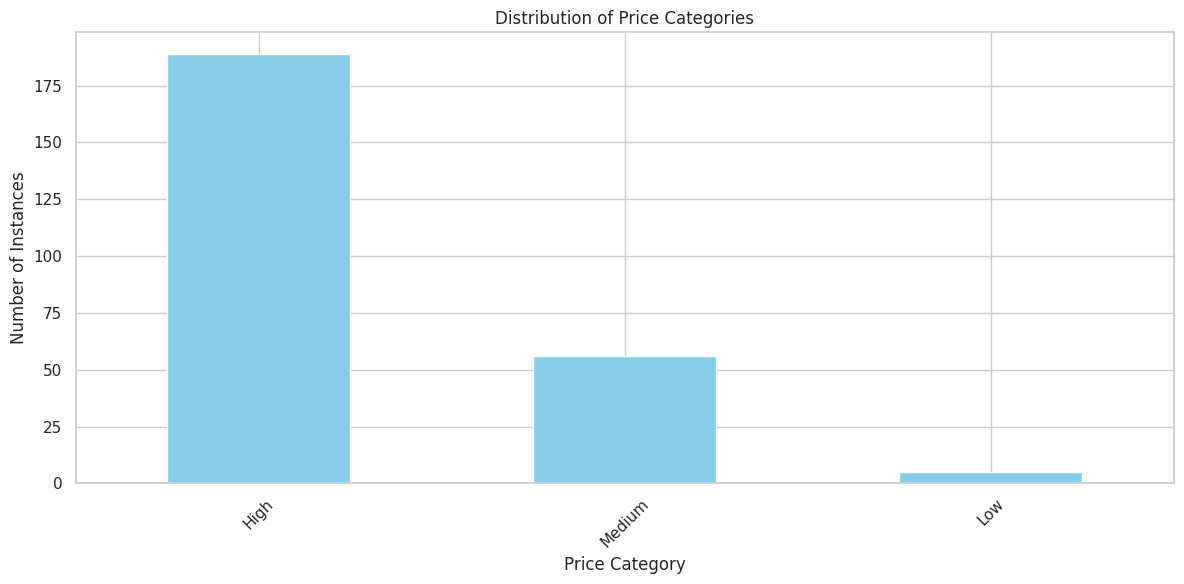
\includegraphics[width=0.9\columnwidth]{gpa_distribution.png}
\caption{Distribution of Academic Performance Categories Before Balancing}
\label{fig:gpa_dist}
\end{figure}

A train-test split of the unadjusted dataset was achieved using a stratified sampling method to ensure that the data in each partition of the train and test sets had the same class distributions as the original dataset to avoid data leakage. Minority classes, \textit{Low} and \textit{Medium} were upsampled with replacement to equalize the number of samples from the minority classes and the majority class using the scikit-learn resample function with ($random\_state = 42$).

\section{Methodology}

\subsection{Feature Transformation and Dimensionality Reduction}
Continuous predictors were $z$-score normalized using StandardScaler, trained on the training partition, and applied to the training and test partitions. Principal Component Analysis (PCA) is used for dimensionality reduction and elimination of multicollinearity. The analysis of the principal components revealed that the (cumulative) explained variance across the feature space was maintained at about 95\% when the top 19 principal components were kept, as shown in Fig.~\ref{fig:pca_analysis}(a). The results from the training samples projected onto the first two principal components, with colors indicating the GPA group, are displayed in Fig.~\ref{fig:pca_analysis}(b).

\begin{figure}[htbp]
\centering
\begin{subfigure}[b]{0.48\columnwidth}
    \centering
    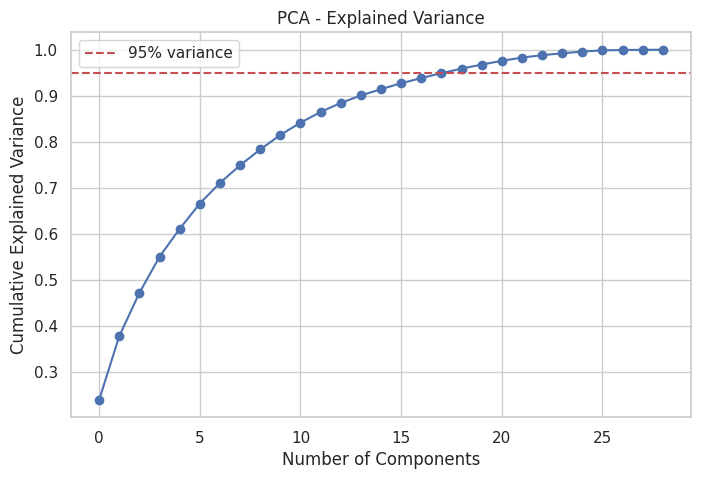
\includegraphics[width=\textwidth]{pca_variance.png}
    \caption{Explained Variance}
    \label{fig:pca_var}
\end{subfigure}
\hfill
\begin{subfigure}[b]{0.48\columnwidth}
    \centering
    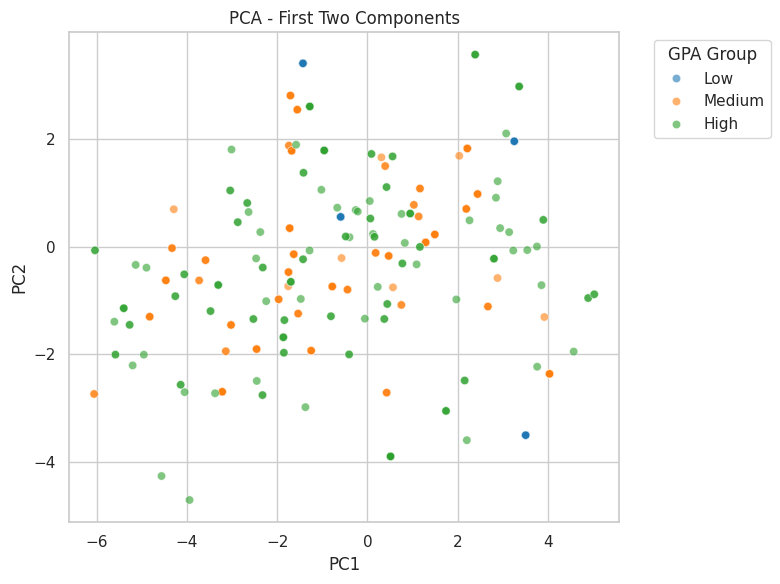
\includegraphics[width=\textwidth]{pca_components.png}
    \caption{First Two Components}
    \label{fig:pca_comp}
\end{subfigure}
\caption{PCA Decomposition Analysis: (a) cumulative explained variance used to select 19 components, and (b) projection of samples onto the first two principal components colored by GPA group.}
\label{fig:pca_analysis}
\end{figure}

\subsection{Supervised Classification Models}
Seven supervised machine learning algorithms were implemented on the PCA-transformed feature representations:
\begin{enumerate}
    \item \textbf{Logistic Regression}: Regularized linear baseline model for multi-class classification with a cross-entropy objective.
    \item \textbf{Decision Tree Classifier}: Set to recursively partition the feature space based on gini impurity to capture non-linear relationships.
    \item \textbf{Random Forest Classifier}: An ensemble of bagged Decision Trees (with $n = 200$ estimators) to achieve generalizability and to mitigate the variance of individual decision trees.
    \item \textbf{XGBoost Classifier}:  A gradient-boosted tree ensemble that fits trees sequentially, each tree tuned to the residual errors of the previous set of trees by a second-order-optimised, regularized objective function, which allows it to fit complex non-linear relationships without overfitting.
    \item \textbf{Support Vector Machine (SVM)}: A margin-maximizing classification method that was used on the PCA-reduced feature space with a kernel transformation to create non-linear decision boundaries between the three tiers of academic performance.
    \item \textbf{Neural Network (Multi-Layer Perceptron)}: A fully connected feed-forward network with hidden layers consisting of non-linear activation functions trained to learn a non-linear mapping from the PCA-transformed behavioral and psychological features to the ordinal GPA category.
    \item \textbf{Gradient Boosting Classifier}: A shallow decision tree scikit-learn boosted ensemble that fits shallow decision trees to the maxmin of the negative multi-class log-loss, which is more conservative in depth of the shallow decision trees than XGBoost and successively reduces the bias.
\end{enumerate}


\subsection{Evaluation Framework}
Model performance was assessed on the unseen test distribution, based on accuracy, precision, recall, F1-score, and AUC-ROC (one-vs-rest) metrics, including macro- and weighted-averaged versions. Note that macro averages assign the same weight to each class, and thus show the performance across each minority class (\textit{Low} and \textit{Medium}), while weighted averages are weighted according to the proportion of the classes in the (imbalanced) test set and thus track the performance more closely with the overall accuracy. Reporting in addition to accuracy allows for a more complete comparison. Multi-class confusion matrices were calculated, and the results are plotted to show misclassification on the borders between individual performance levels.

\section{Results and Discussion}
In this section, we discuss the findings of our preditive models and analyze the influence of behavoiur, lifestyle and mental health related features on student academic performance [2]. The models were evaluated on the test dataset using standard classification metrics, including accuracy, precision, recall and F1-score.

\subsection{Feature Importance and Dependency Analysis}
To find the relationships between the behavioral and mental metrics, a correlation matrix was created across all numerical predictors, shown in Fig.~\ref{fig:heatmap}. The correlation matrix shows that the variables related to mental health and behavioral regulation like stress\_score, anxiety\_level, loneliness\_score, and dopamine\_dependency\_index  clustered closely together and demonstrated direct link to addiction\_score and mental\_health\_risk\_score [1, 3]

\begin{figure*}[htbp]
\centering
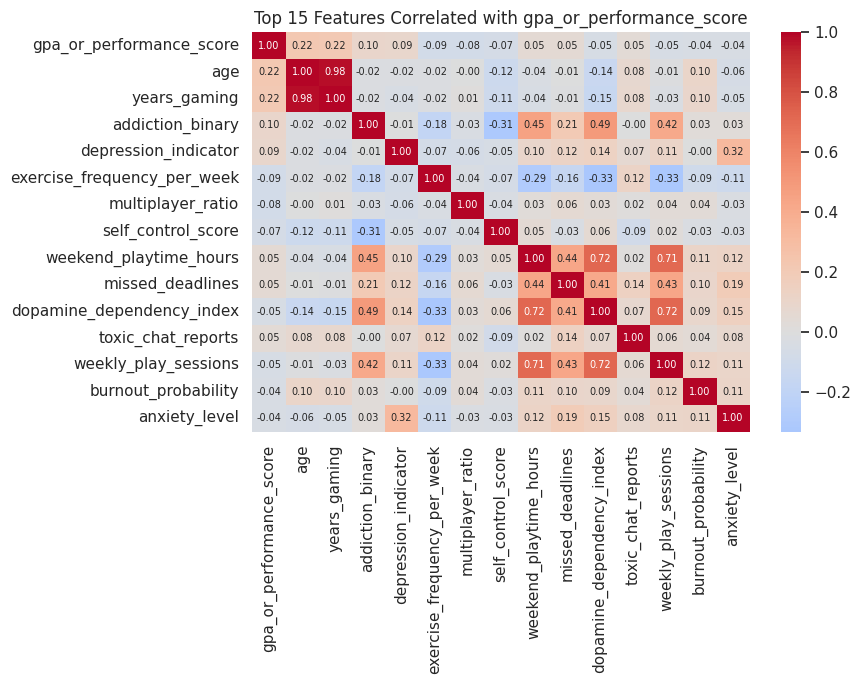
\includegraphics[width=0.9\textwidth]{correlation_heatmap.png}
\caption{Correlation Heatmap of Behavioral, Psychological, and Academic Features}
\label{fig:heatmap}
\end{figure*}

However, the linear correlation between gameplay  duration metrics and GPA scores were weak, confiirming with contradictions in prior literature [1]. Conseqently, non-linear feature ranking with tree-based models and PCA loading components was used to isolate primary determinants [2]. The most influential attributes affecting academic tier differentiation were found to be dopamine\_dependency\_index, consecutive\_hours\_max, late\_night\_sessions\_hours, and productivity\_drop\_percent. Late-night seesions and consecutive gaming hours showed a significant affect on early principal components, explaining variances associated with student performance degradation [1,3]


\subsection{Model Performance Metrics}
The seven classifier models run were Decision Tree, Logistic Regression, Random Forest, XGBoost, SVM, Neural Network, and Gradient Boosting. They were trained on a balanced PCA feature representation and evaluated against the original imbalanced test split.
Table~\ref{tab:performance} shows the comparative metrics for both macro and weighted averages for accuracy, precision, recall, F1-score and AUC-ROC for all the models.

\begin{table*}[htbp]
\caption{Performance Metrics (Macro and Weighted) for All Seven Classifiers}
\label{tab:performance}
\centering
\footnotesize
\begin{tabular}{|l|c|c|c|c|c|c|c|c|c|}
\hline
\multirow{2}{*}{Model} & \multirow{2}{*}{Accuracy} & \multicolumn{2}{c|}{Precision} & \multicolumn{2}{c|}{Recall} & \multicolumn{2}{c|}{F1-Score} & \multicolumn{2}{c|}{AUC-ROC} \\
\cline{3-10}
 & & Macro & Weighted & Macro & Weighted & Macro & Weighted & Macro & Weighted \\
\hline
Decision Tree       & 0.5600 & 0.3321 & 0.6373 & 0.3317 & 0.5600 & 0.3238 & 0.5894 & 0.5309 & 0.5592 \\
\hline
Logistic Regression & 0.4400 & 0.3119 & 0.5883 & 0.3006 & 0.4400 & 0.2838 & 0.4834 & 0.5969 & 0.4711 \\
\hline
Random Forest        & 0.7200 & 0.3687 & 0.6606 & 0.3589 & 0.7200 & 0.3549 & 0.6820 & 0.6838 & 0.5661 \\
\hline
XGBoost               & 0.7600 & 0.4142 & 0.7129 & 0.3979 & 0.7600 & 0.3992 & 0.7301 & 0.6787 & 0.5392 \\
\hline
SVM                   & 0.5800 & 0.3174 & 0.6224 & 0.3190 & 0.5800 & 0.3148 & 0.5978 & 0.6620 & 0.5164 \\
\hline
Neural Network        & 0.5600 & 0.3437 & 0.6551 & 0.3533 & 0.5600 & 0.3330 & 0.5905 & 0.6369 & 0.5773 \\
\hline
Gradient Boosting     & 0.7000 & 0.3131 & 0.6239 & 0.3285 & 0.7000 & 0.3156 & 0.6561 & 0.6887 & 0.6201 \\
\hline
\end{tabular}
\end{table*}

Among the classes \textbf{XGBoost} achieved the highest overall accuracy of 76\% and the highest macro F1-score of 0.3992, demonstrating the benefit of sequential, gradient-corrected boosting models the non-linear interactions between behavioral and mental predictors. \textbf{Random Forest} was the second best with an accuracy of 72.00\% and a macro F1-score of 0.3549, again demonstrating the benefit of ensemble bagging in reducing variance over noisy behavioral attributes [2]. \textbf{Gradient Boosting} performed comparably with an accuracy of 70\% and a F1-score of 0.3156, suggesting that conservative estimator favoured the major \textit{High} class. 
 \textbf{Decision Tree} and \textbf{Neural Network} both reached 56.00\% accuracy, while \textbf{SVM} reached 58.00\% accuracy. All of the single tree based classifier, feed-forward network and a kernel-based margin classifier struggled to match the other methods. \textbf{Logistic Regression} reached the lowest accuracy of 44.00\% showiung thatt the linear boundaries were insufficient for this dataset.

 Because the test set was kept imbalanced, the weighted averaged metrics in Table~\ref{tab:performance} are consistently higher than its macro averages since weighted average is dominated by the performance of \textit{High} class. \textbf{XGBoost} leads on weighted precision (.7129) and f1-score (0.7301), while \textbf{Gradient Boosting} and \textbf{Random Forest} show a comparative F1-score (0.6561 and 0.6820) despite their moderate macro F1-score. This divergence between macro and weighted average shows that although the top models classify the majority \textit{High}-performing students accurately, all seven classifiers still struggle to reliably identify the minority \textit{Low}- and \textit{Medium}-performing students, which is a more actionable subgroup for the academic early-warning system.

Fig.~\ref{fig:combined_results}(a) shows the multi-class confusion matrices for all seven classifiers. Analyzing them shows the missclasifications primarily occured between adjacent performance groups (\textit{Medium} vs. \textit{Low} or \textit{Medium} vs. \textit{High}), rather than the extremes (\textit{Low} vs. \textit{High}). A pattern that showed up consistently across all models. This pattern reflects the progressive nature of academic decline, where moderate gamin interference produces small shifts in-between adjacent GPA bands [1].

Per-class discrimination ability was further shown by using one-vs-rest ROC curves, shown in Fig.~\ref{fig:combined_results}(b). Notably, the overall accuracy favoured \textbf{XGBoost}, several models achieved strong isolation of the minority \textit{Low}-performance tier. The AUC of both the \textbf{XGBoost} and \textbf{SVM} models reached 1.00, \textbf{Random Forest} reached 0.92, \textbf{Gradient Boosting} reached 0.88, and \textbf{Logistic Regression} reached 0.82 all substantially higher than the \textit{Low}-class AUC of the \textbf{Decision Tree} (0.49), suggesting that ensemble and margin-based methods are better suited for flagging the minority low-performing students even when their aggregate multi-class accuracy is lower.


\subsection{AUC-ROC Discriminative Analysis}
To supplement the threshold-dependent merics, the area under the receiver operating characteristic curve (AUC-ROC) was analyzed to assess the intrinsic discriminative capability of each model across different varying decision boundaries. The macro-averaged AUC scores revealed that, models that used some sort of boosting achieved the highest macro AUC \textbf{Gradient Boosting} (0.6887)
,\textbf{Random Forest} (0.6838) and \textbf{XGBoost} (0.6787). With \textbf{SVM} (0.6620), \textbf{Neural Network} (0.6369), and \textbf{Logistic Regression} (0.5969) trailing behind, while the \textbf{Decision Tree} recorded the lowest macro AUC (0.5309) [2]. When weighted by class support, \textbf{Gradient Boosting} was once again the highest with 0.6201, ahead of \textbf{Neural Network} (0.5773), \textbf{Random Forest} (0.5661), \textbf{Decision Tree} (0.5592), \textbf{XGBoost} (0.5392), \textbf{SVM} (0.5164), and \textbf{Logistic Regression} (0.4711). This disparity shows the trade-off inherent to class-imbalanced multi-tier evaluation, while XGBosst maximized overall top-1 label accuracy, its soft-probability margins were somewhat compressed relative to Graient Boosting and Random Forest once minority-class upsampling variance and class weighting were accounted for [1, 2]. The boosted models collectively provided more cosistent true-positive tracking at low false-positive rates than other models,  supporting their continued preference for high-risk student flagging tasks [1, 2]. Fig.~\ref{fig:combined_results}(c) combines the three headline metrics accuracy, weighted F1-score, and weighted AUC-ROC across all seven models. It shows XGBoost and Gradient Boosting leading on accuracy and F1-score, while Gradient Boosting leads on weighted AUC-ROC, with Random Forest a consistent runner-up across all three metrics.

\begin{figure*}[htbp]
\centering
\begin{subfigure}[b]{\textwidth}
    \centering
    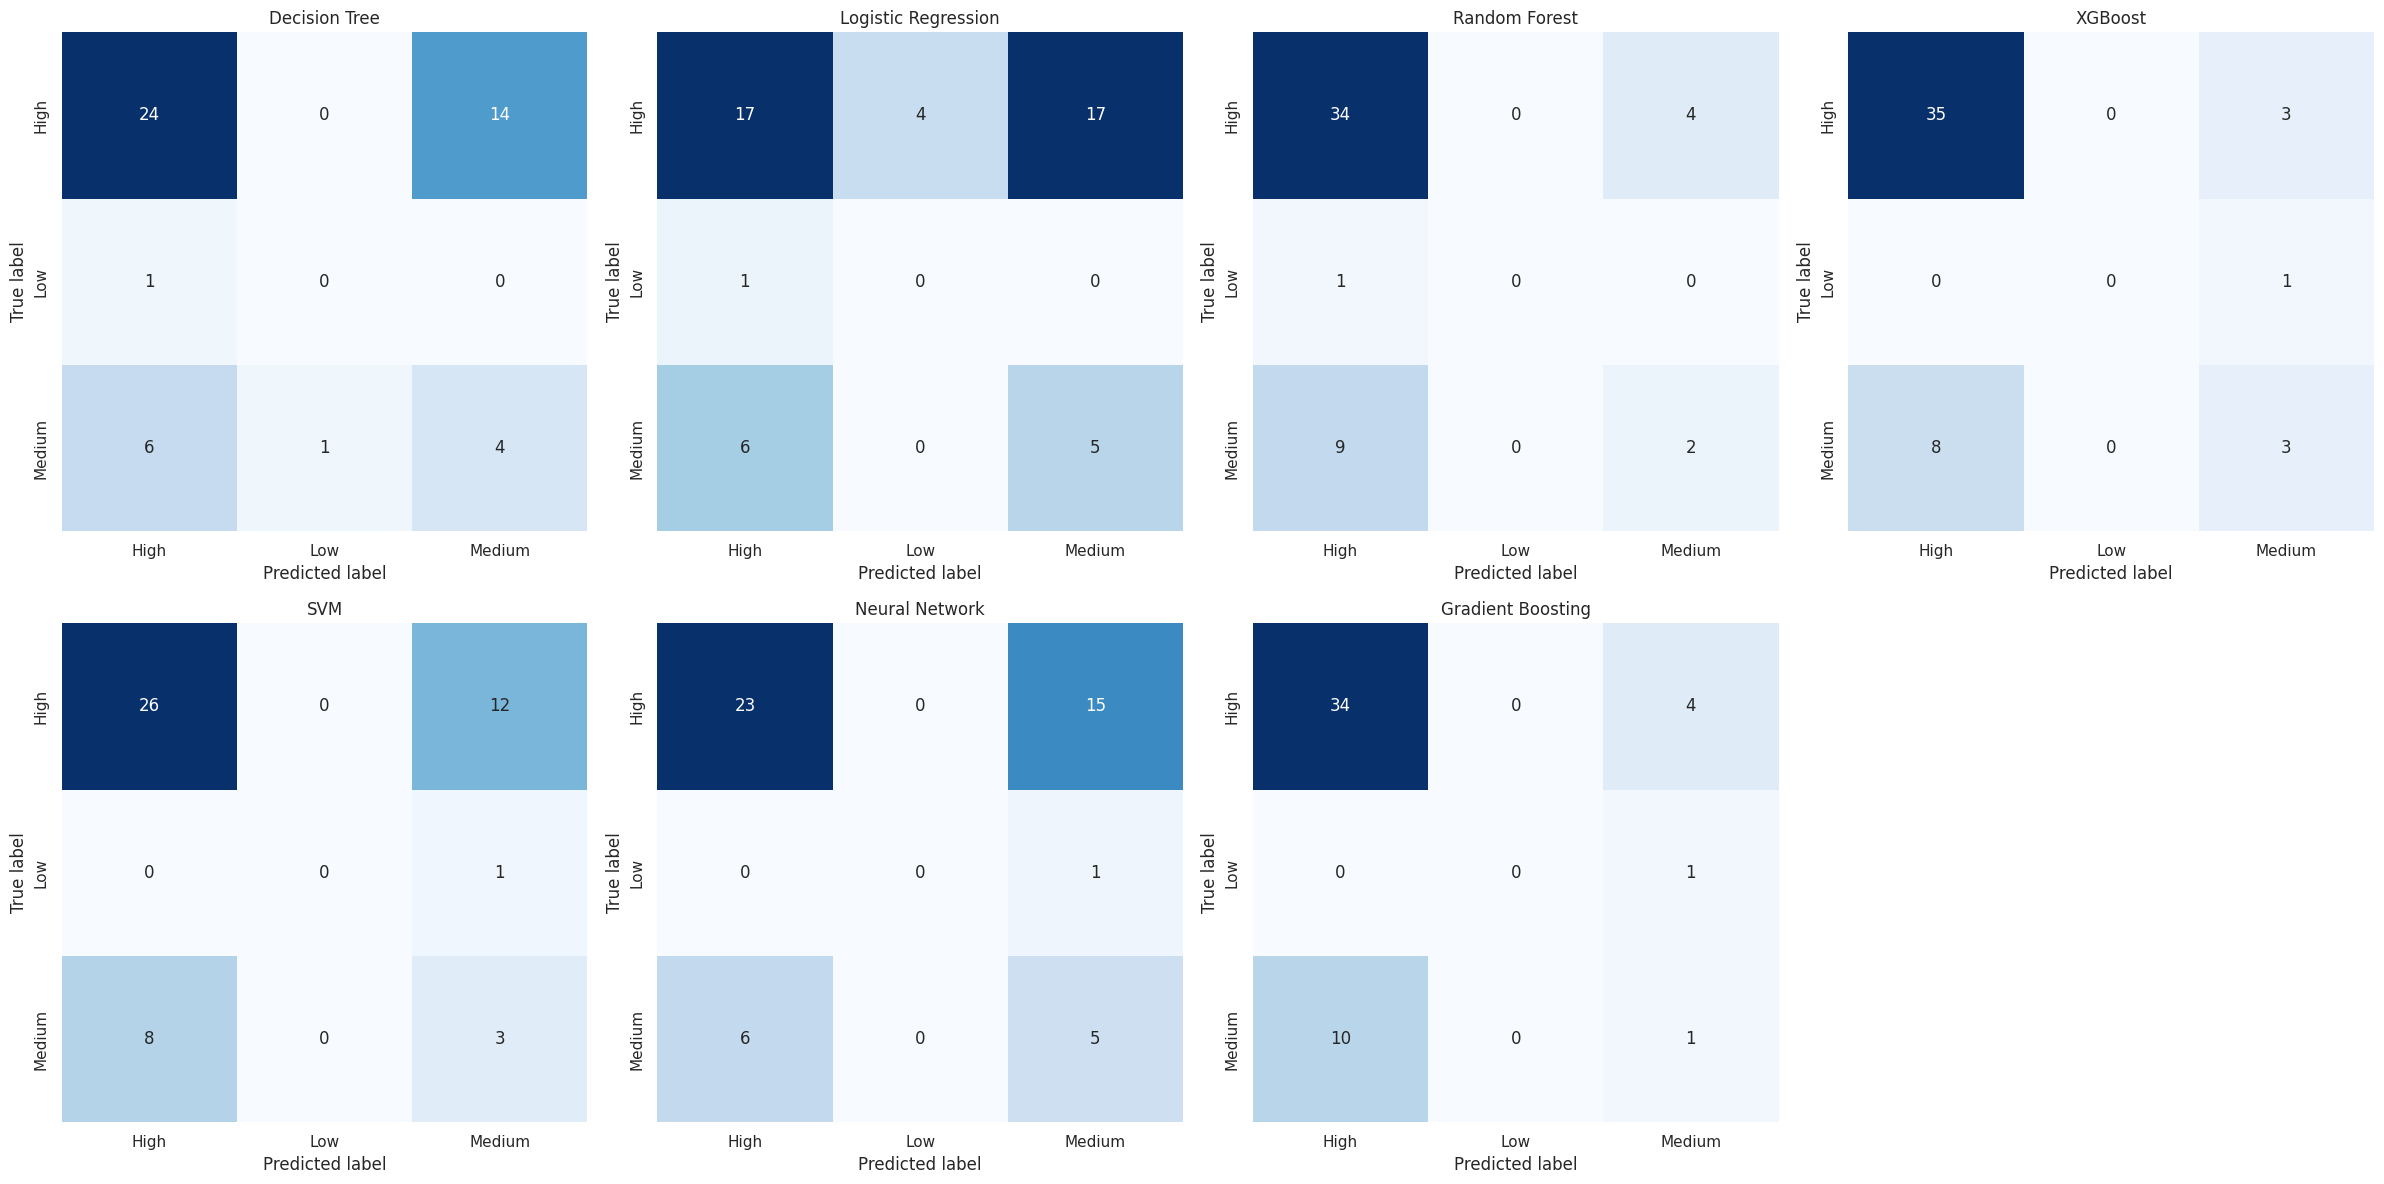
\includegraphics[width=0.85\textwidth,height=0.28\textheight,keepaspectratio]{confusion_matrices.png}
    \caption{Confusion Matrices for all seven classifiers}
    \label{fig:confusion_matrices}
\end{subfigure}

\vspace{2mm}
\begin{subfigure}[b]{\textwidth}
    \centering
    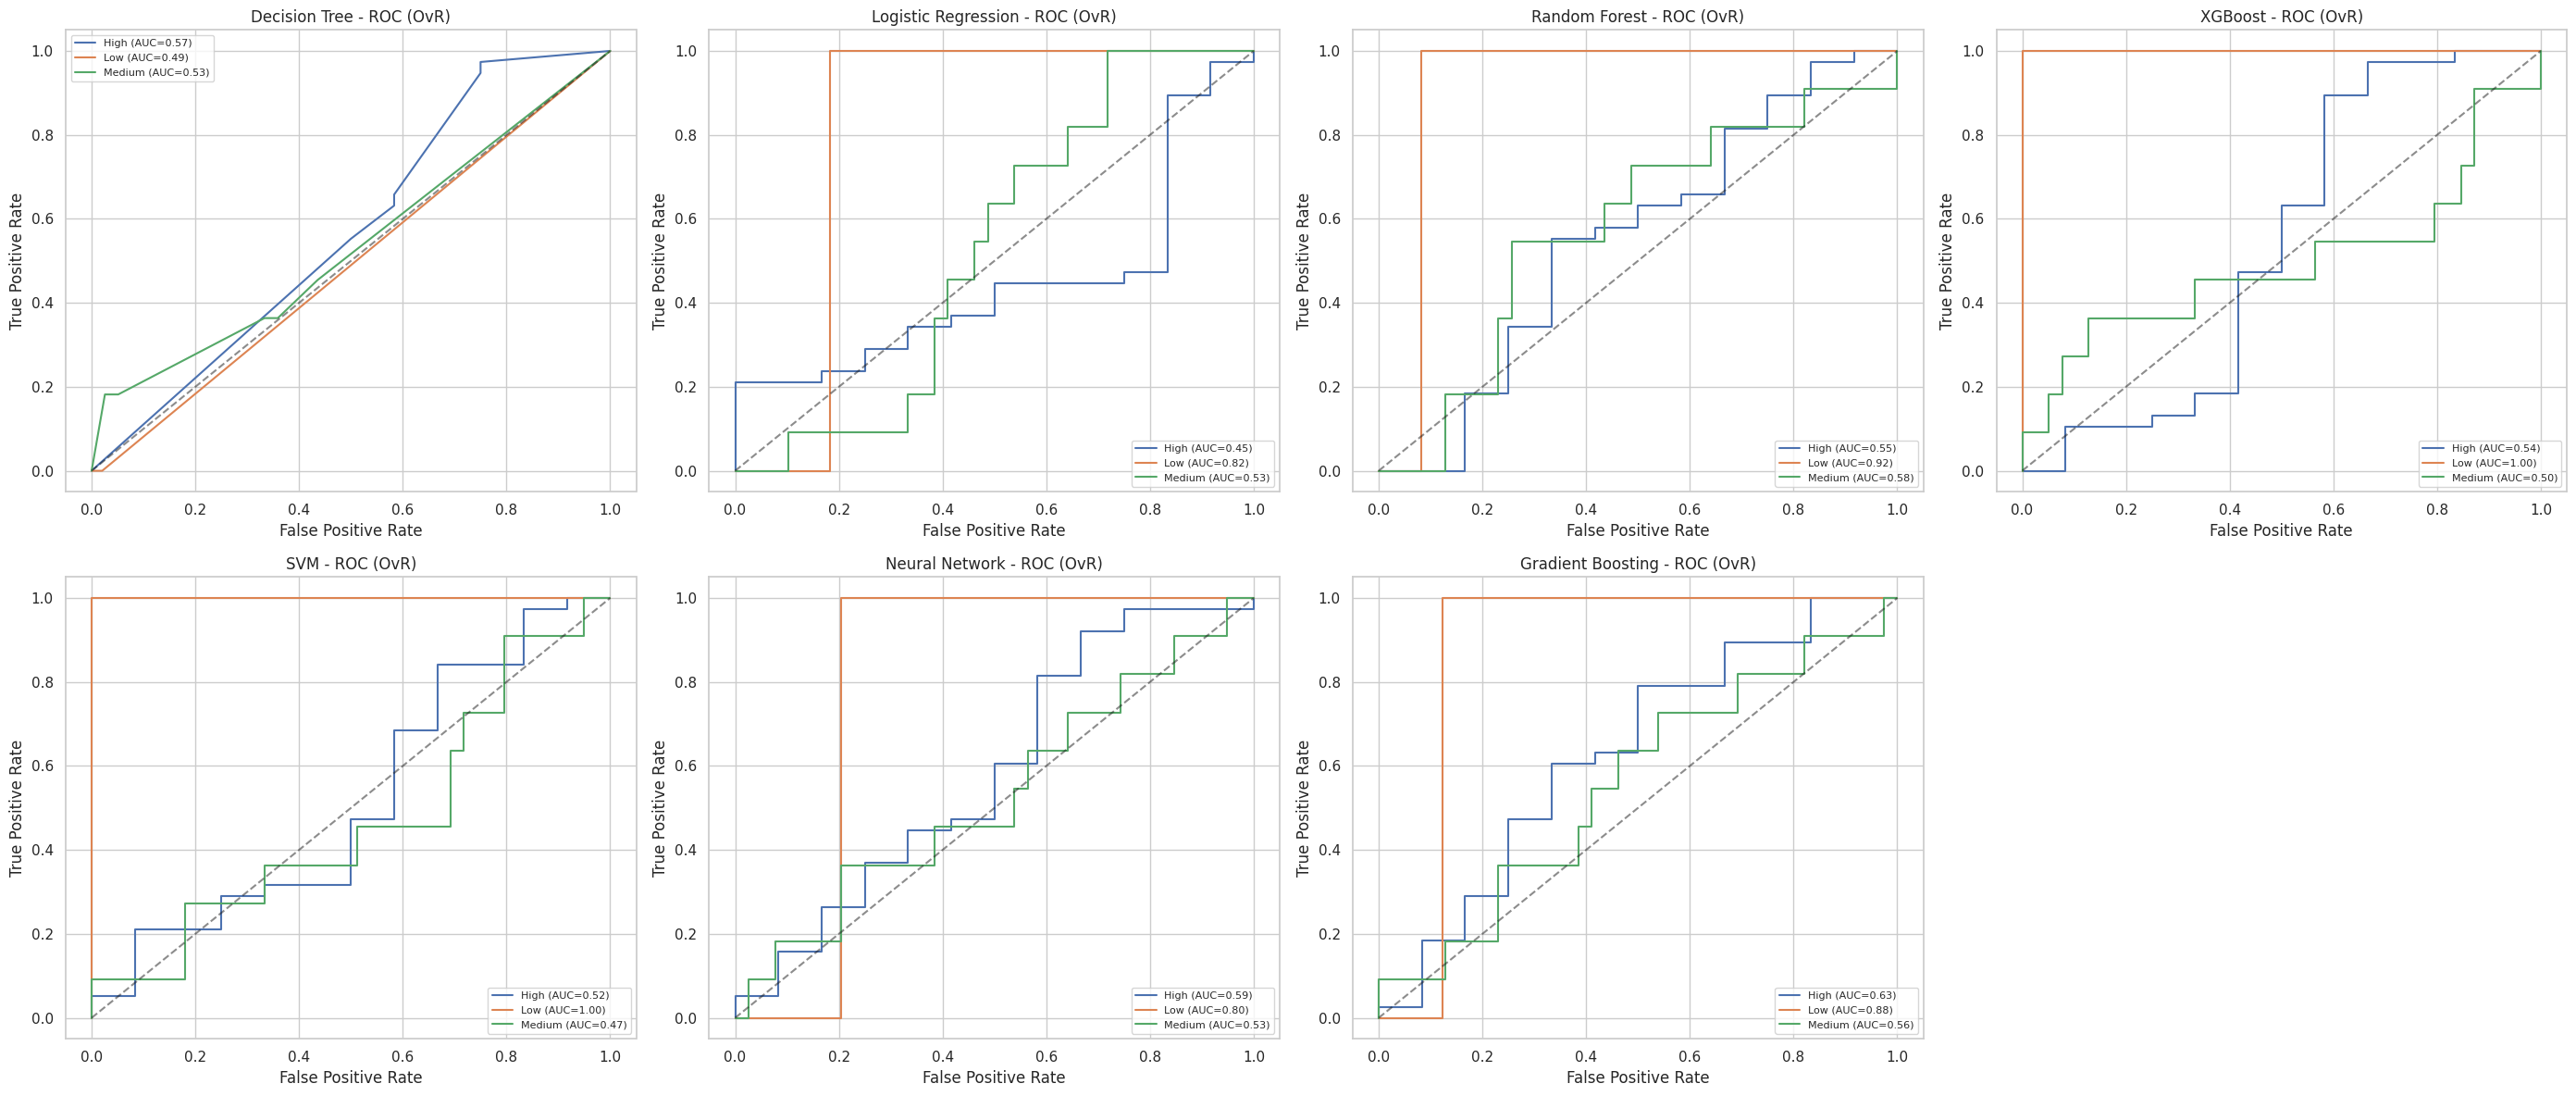
\includegraphics[width=0.85\textwidth,height=0.28\textheight,keepaspectratio]{roc_curves.png}
    \caption{One-vs-Rest ROC Curves for all seven classifiers}
    \label{fig:roc_curves}
\end{subfigure}

\vspace{2mm}
\begin{subfigure}[b]{0.55\textwidth}
    \centering
    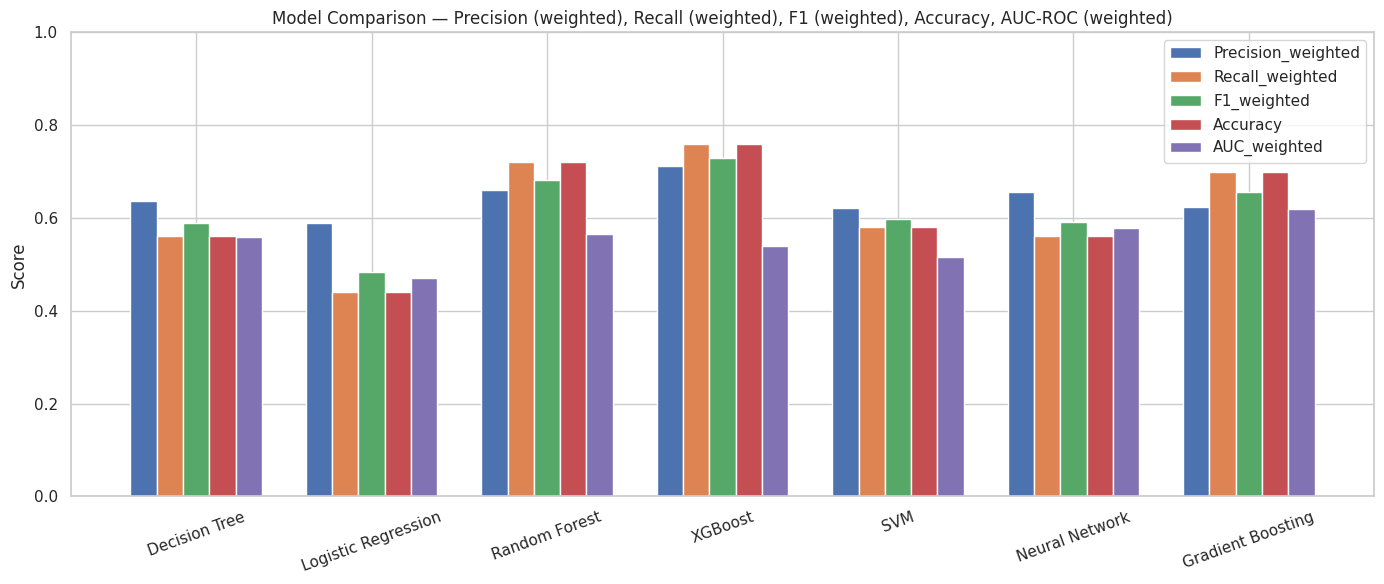
\includegraphics[width=\textwidth,height=0.2\textheight,keepaspectratio]{model_comparison.png}
    \caption{Accuracy, weighted F1-score, and weighted AUC-ROC across all seven models}
    \label{fig:model_comparison}
\end{subfigure}
\caption{Combined model evaluation visualizations: (a) confusion matrices, (b) one-vs-rest ROC curves, and (c) comparative accuracy/F1/AUC-ROC summary for Decision Tree, Logistic Regression, Random Forest, XGBoost, SVM, Neural Network, and Gradient Boosting classifiers.}
\label{fig:combined_results}
\end{figure*}

\FloatBarrier

\section{Conclusion}

\subsection{Key Findings}
The results provide a clear answer to the central question of this study: academic performance is measurably related to \emph{how} students game, not to how much they game. Raw playtime metrics such as daily\_playtime\_hours showed only a weak linear correlation with GPA, consistent with the mixed findings in prior literature, but a distinct cluster of behavioral and psychological indicators dopamine\_dependency\_index, consecutive\_hours\_max, late\_night\_sessions\_hours, and productivity\_drop\_percent emerged as the strongest and most consistent predictors of academic tier. The results shows that some factors such as late-night, uninterupted gaming sessions affect the academic performance instead of total hours spent during gaming. Furthermore, the confusion matrix shows continuous rather than discrete relationship: errors occurred almost entirely between adjacent tiers (\textit{Low}$\leftrightarrow$\textit{Medium}, \textit{Medium}$\leftrightarrow$\textit{High}), never between the extremes, consistent with academic decline unfolding gradually rather than in sudden jumps.

On the question of predictability, the answer is a qualified yes. \textbf{XGBoost} was able to classify a student's academic performance tier from gaming with 76\% overall accuracy, and together with \textbf{SVM} it achieved a perfect 1.00 AUC in isolating the minority \textit{Low}-performance tier, specifically indicating that genuinely at-risk students, when present in the data, could be reliably picked out from the rest. At the same time, the modest macro F1-scores across all seven models (0.28--0.40) reveal that this predictive strength is not uniform: models are focusing accurately on the majority \textit{High}-performing group but cannot perform well when it comes to separating the \textit{Low} and \textit{Medium} tiers from each other. Taken together, the results suggest that gaming behavior, particularly its compulsivity and timing carries a real, learnable signal about academic risk, and that ensemble models such as XGBoost and Gradient Boosting can recognize that signal well enough to point out students who are at risk, though not very accurate to replace individualized follow-up. 

\subsection{Shortcomings}
Several limitations temper these findings. The dataset is small (n=250), self-reported, cross-sectional, and drawn from a single source, which restricts statistical power and prevents any causal interpretation of the observed relationships. There is also a consistent gap between weighted and macro-averaged metrices in all seven models that were run. Every model still struggles to identify the minority \textit{Low}- and \textit{Medium}-performing students even though the accuracy looks trustworthy. Finally, as the features were not passively logged usage data but behavioral self-reports, we cannot exclude social desirability bias and measurement errors.

\subsection{Future Work}
Building on these limitations, future research work should figure out how to replace self-report with passive usage telemetry, pursue multi-institutional and longitudinal validation to assess both generalizability and causal ordering. It should also aim to reduce the macro/weighted performance gap. In conclusion, of all the approaches used here, gradient-boosted ensembles stand out as the most effective for gaming-related academic early-warning systems, but in practice, choosing a model shouldn't be based on accuracy alone; rather, how well it catches the minority class and confidence scores matter too.  

\begin{thebibliography}{00}
\bibitem{tas2019} I. Ta\c{s}, ``Relationship between Internet Addiction, Gaming Addiction and School Engagement among Adolescents,'' \textit{Universal Journal of Educational Research}, vol. 5, no. 12, pp. 2304--2311, 2017.
\bibitem{shukry2021} A. I. Mohd Shukry \textit{et al.}, ``Gaming Addiction and Academic Performance: A Battle for Student Success,'' \textit{Journal of Islamic, Social, Economics and Development (JISED)}, vol. 9, no. 66, pp. 698--706, 2024.
\bibitem{wright2011} J. Wright, ``The Effects of Video Game Play on Academic Performance,'' \textit{Modern Psychological Studies}, vol. 17, no. 1, pp. 37--44, 2011.
\bibitem{mahmud2020} S. Mahmud \textit{et al.}, ``Online Gaming and Its Effect on Academic Performance of Bangladeshi University Students: A Cross-Sectional Study,'' \textit{Health Science Reports}, vol. 6, e1774, 2023.
\bibitem{anjum2021} R. Anjum, N. H. Nodi, P. R. Das, A. S. M. Roknuzzaman, R. Sarker, and M. R. Islam, ``Exploring the association between online gaming addiction and academic performance among the school-going adolescents in Bangladesh: A cross-sectional study,'' \textit{Health Science Reports}, vol. 7, no. 9, e70043, 2024.
\bibitem{alzahrani2023} A. K. D. Alzahrani and M. D. Griffiths, ``Problematic gaming and students' academic performance: A systematic review,'' \textit{International Journal of Mental Health and Addiction}, vol. 23, no. 5, pp. 4062--4095, 2025.
\bibitem{jiang2014} Q. Jiang, ``Internet addiction among young people in China: Internet connectedness, online gaming, and academic performance decrement,'' \textit{Internet Research}, vol. 24, no. 1, pp. 2--20, 2014, doi: 10.1108/IntR-01-2013-0004.
\bibitem{reysen2021} R. Reysen, R. Balkin, and A. Winburn, ``Predicting academic entitlement for college students on academic probation using factors of life balance and gaming addiction,'' \textit{College Teaching}, vol. 72, no. 2, pp. 126--134, 2024.
\end{thebibliography}

\end{document}